
    \begin{figure}[H]
      {
        \setlength{\tabcolsep}{3.0pt}
        \setlength\cmidrulewidth{\lightrulewidth} % Make cmidrule = 
        \begin{adjustbox}{width=0.5cm,center}
          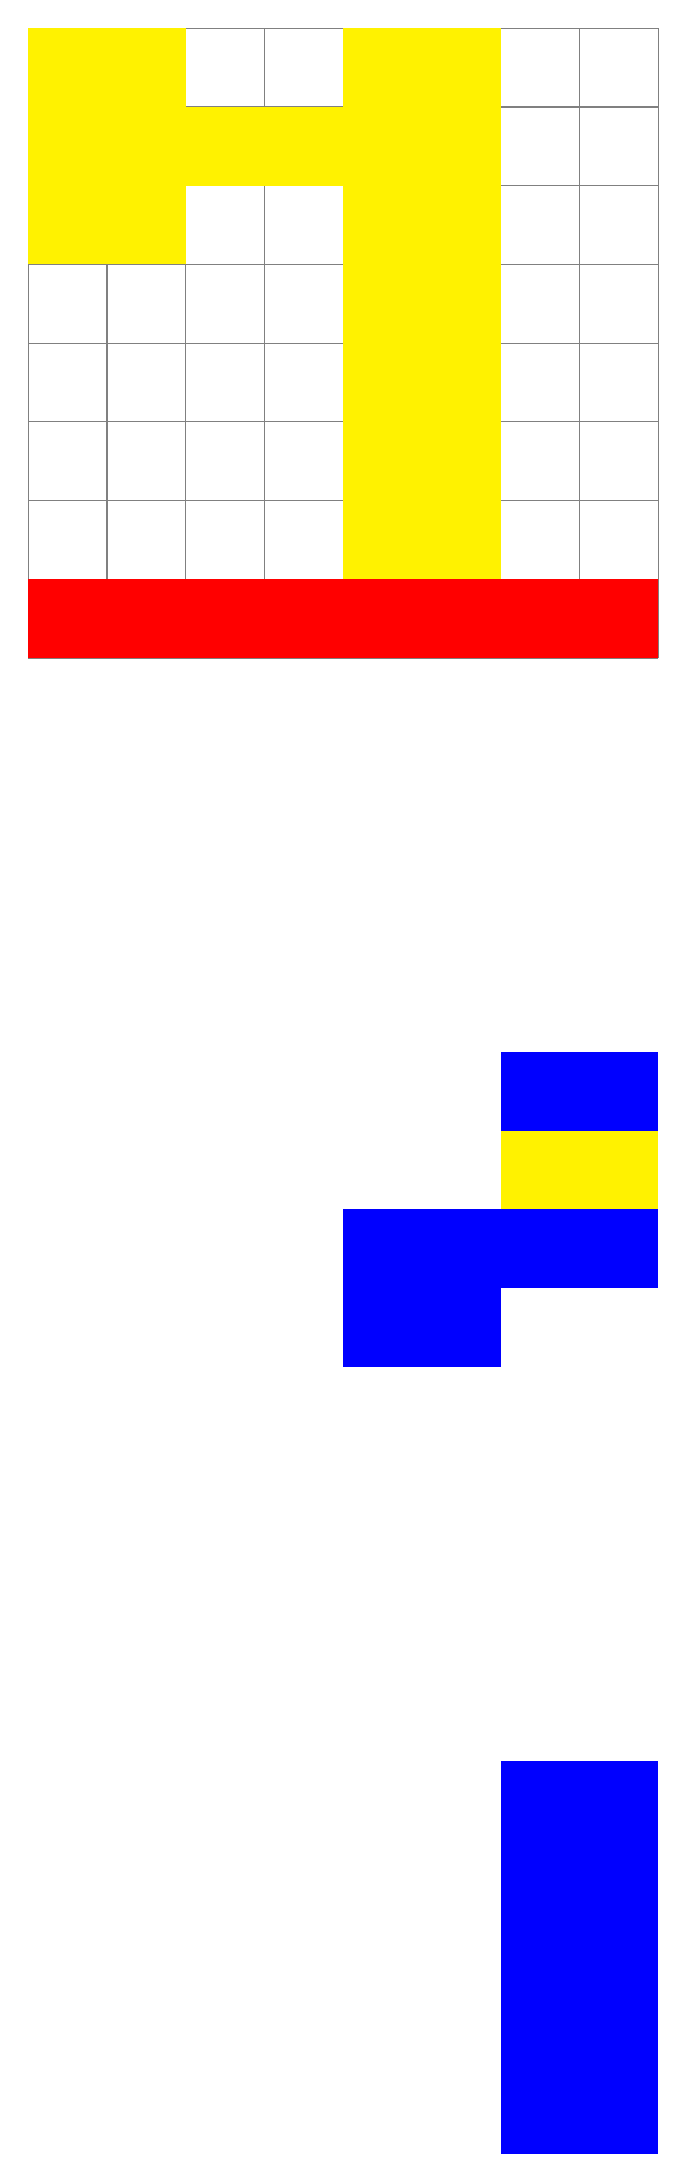
\begin{tikzpicture}
    
\def\BACKGROUNDONE{yellow}
\def\BACKGROUNDTWO{blue}
\def\CHARCOLOR{red}
	\draw[step=1.0,gray,thin] (0,0) grid (8,8);
	\fill[\BACKGROUNDONE] (0,7) rectangle ++ (1,1);
	\fill[\BACKGROUNDONE] (1,7) rectangle ++ (1,1);
	\fill[\BACKGROUNDONE] (4,7) rectangle ++ (1,1);
	\fill[\BACKGROUNDONE] (5,7) rectangle ++ (1,1);
	\fill[\BACKGROUNDONE] (0,6) rectangle ++ (1,1);
	\fill[\BACKGROUNDONE] (1,6) rectangle ++ (1,1);
	\fill[\BACKGROUNDONE] (2,6) rectangle ++ (1,1);
	\fill[\BACKGROUNDONE] (3,6) rectangle ++ (1,1);
	\fill[\BACKGROUNDONE] (4,6) rectangle ++ (1,1);
	\fill[\BACKGROUNDONE] (5,6) rectangle ++ (1,1);
	\fill[\BACKGROUNDONE] (0,5) rectangle ++ (1,1);
	\fill[\BACKGROUNDONE] (1,5) rectangle ++ (1,1);
	\fill[\BACKGROUNDONE] (4,5) rectangle ++ (1,1);
	\fill[\BACKGROUNDONE] (5,5) rectangle ++ (1,1);
	\fill[\BACKGROUNDONE] (4,4) rectangle ++ (1,1);
	\fill[\BACKGROUNDONE] (5,4) rectangle ++ (1,1);
	\fill[\BACKGROUNDONE] (4,3) rectangle ++ (1,1);
	\fill[\BACKGROUNDONE] (5,3) rectangle ++ (1,1);
	\fill[\BACKGROUNDONE] (4,2) rectangle ++ (1,1);
	\fill[\BACKGROUNDONE] (5,2) rectangle ++ (1,1);
	\fill[\BACKGROUNDONE] (4,1) rectangle ++ (1,1);
	\fill[\BACKGROUNDONE] (5,1) rectangle ++ (1,1);
	\fill[\CHARCOLOR] (0,0) rectangle ++ (1,1);
	\fill[\CHARCOLOR] (1,0) rectangle ++ (1,1);
	\fill[\CHARCOLOR] (2,0) rectangle ++ (1,1);
	\fill[\CHARCOLOR] (3,0) rectangle ++ (1,1);
	\fill[\CHARCOLOR] (4,0) rectangle ++ (1,1);
	\fill[\CHARCOLOR] (5,0) rectangle ++ (1,1);
	\fill[\CHARCOLOR] (6,0) rectangle ++ (1,1);
	\fill[\CHARCOLOR] (7,0) rectangle ++ (1,1);
	\fill[\BACKGROUNDTWO] (6,-6) rectangle ++ (1,1);
	\fill[\BACKGROUNDTWO] (7,-6) rectangle ++ (1,1);
	\fill[\BACKGROUNDONE] (6,-7) rectangle ++ (1,1);
	\fill[\BACKGROUNDONE] (7,-7) rectangle ++ (1,1);
	\fill[\BACKGROUNDTWO] (4,-8) rectangle ++ (1,1);
	\fill[\BACKGROUNDTWO] (5,-8) rectangle ++ (1,1);
	\fill[\BACKGROUNDTWO] (6,-8) rectangle ++ (1,1);
	\fill[\BACKGROUNDTWO] (7,-8) rectangle ++ (1,1);
	\fill[\BACKGROUNDTWO] (4,-9) rectangle ++ (1,1);
	\fill[\BACKGROUNDTWO] (5,-9) rectangle ++ (1,1);
	\fill[\BACKGROUNDTWO] (6,-15) rectangle ++ (1,1);
	\fill[\BACKGROUNDTWO] (7,-15) rectangle ++ (1,1);
	\fill[\BACKGROUNDTWO] (6,-16) rectangle ++ (1,1);
	\fill[\BACKGROUNDTWO] (7,-16) rectangle ++ (1,1);
	\fill[\BACKGROUNDTWO] (6,-17) rectangle ++ (1,1);
	\fill[\BACKGROUNDTWO] (7,-17) rectangle ++ (1,1);
	\fill[\BACKGROUNDTWO] (6,-18) rectangle ++ (1,1);
	\fill[\BACKGROUNDTWO] (7,-18) rectangle ++ (1,1);
	\fill[\BACKGROUNDTWO] (6,-19) rectangle ++ (1,1);
	\fill[\BACKGROUNDTWO] (7,-19) rectangle ++ (1,1);

          \end{tikzpicture}
        \end{adjustbox}
      }\caption*{\$7F}
    \end{figure}
    